%% Commands for TeXCount
%TC:macro \cite [option:text,text]
%TC:macro \citep [option:text,text]
%TC:macro \citet [option:text,text]
%TC:envir table 0 1
%TC:envir table* 0 1
%TC:envir tabular [ignore] word
%TC:envir displaymath 0 word
%TC:envir math 0 word
%TC:envir comment 0 0

\documentclass[sigconf, authordraft]{acmart}


\AtBeginDocument{%
\providecommand{\BibTeX}{{%
\normalfont B\kern-0.5em{\scshape i\kern-0.25em b}\kern-0.8em\TeX}}}

\setcopyright{acmcopyright}
\copyrightyear{2018}
\acmYear{2018}
\acmDOI{XXXXXXX.XXXXXXX}

\acmConference[Conference
acronym
'XX]{Make sure to enter the correct conference title from your rights confirmation emai}{June 03--05, 2018}{Woodstock, NY}

\acmPrice{15.00}
\acmISBN{978-1-4503-XXXX-X/18/06}

%%\acmSubmissionID{123-A56-BU3}

\settopmatter{printacmref=true}
%%
%% For managing citations, it is recommended to use bibliography
%% files in BibTeX format.
%%
%% You can then either use BibTeX with the ACM-Reference-Format style,
%% or BibLaTeX with the acmnumeric or acmauthoryear sytles, that include
%% support for advanced citation of software artefact from the
%% biblatex-software package, also separately available on CTAN.
%%
%% Look at the sample-*-biblatex.tex files for templates showcasing
%% the biblatex styles.
%%

%%
%% For managing citations, it is recommended to use bibliography
%% files in BibTeX format.
%%
%% You can then either use BibTeX with the ACM-Reference-Format style,
%% or BibLaTeX with the acmnumeric or acmauthoryear sytles, that include
%% support for advanced citation of software artefact from the
%% biblatex-software package, also separately available on CTAN.
%%
%% Look at the sample-*-biblatex.tex files for templates showcasing
%% the biblatex styles.
%%

%%
%% The majority of ACM publications use numbered citations and
%% references.  The command \citestyle{authoryear} switches to the
%% "author year" style.
%%
%% If you are preparing content for an event
%% sponsored by ACM SIGGRAPH, you must use the "author year" style of
%% citations and references.
%% Uncommenting
%% the next command will enable that style.
%%\citestyle{acmauthoryear}

%%
%% end of the preamble, start of the body of the document source.

\usepackage{tabularx}
\begin{document}
	%%
	%% The "title" command has an optional parameter,
	%% allowing the author to define a "short title" to be used in page headers.
	\title{A Uniswap-Powered Decentralized Exchange for Carbon Trading}


	%%
	%% The "author" command and its associated commands are used to define
	%% the authors and their affiliations.
	%% Of note is the shared affiliation of the first two authors, and the
	%% "authornote" and "authornotemark" commands
	%% used to denote shared contribution to the research.
	\author{Wenqin ZHANG, Mingze GONG}


	%%
	%% By default, the full list of authors will be used in the page
	%% headers. Often, this list is too long, and will overlap
	%% other information printed in the page headers. This command allows
	%% the author to define a more concise list
	%% of authors' names for this purpose.
	\renewcommand{\shortauthors}{Trovato and Tobin, et al.}


	%%
	%% The abstract is a short summary of the work to be presented in the
	%% article.
	\begin{abstract}
This project capitalizes on the emergent popularity of carbon-related trading products. Our report commences with a thorough introduction of the project, followed by a detailed delineation of its design structure and the intricacies of the underlying blockchain architecture. We
		also expound upon the nature and prominence of carbon trading products in
		China, which constitute the principal commodities of our exchange. In
		addition to trading, we posit that our platform can significantly contribute
		to the field of carbon finance, with an emphasis on carbon pricing. The utilization
		of blockchain technology and decentralized exchanges in carbon finance presents
		unprecedented potential in terms of efficiency, transparency, and accessibility.
		While the project is currently underway, this paper serves as a comprehensive
		overview of our progress thus far, highlighting the unique contributions
		that the project has already made and outlining the future avenues of work
		and potential expansions.
	\end{abstract}

	\keywords{Uniswap, Decentralized Exchange, Carbon Trading, Smart Contract}

	\begin{teaserfigure}
		\centering
		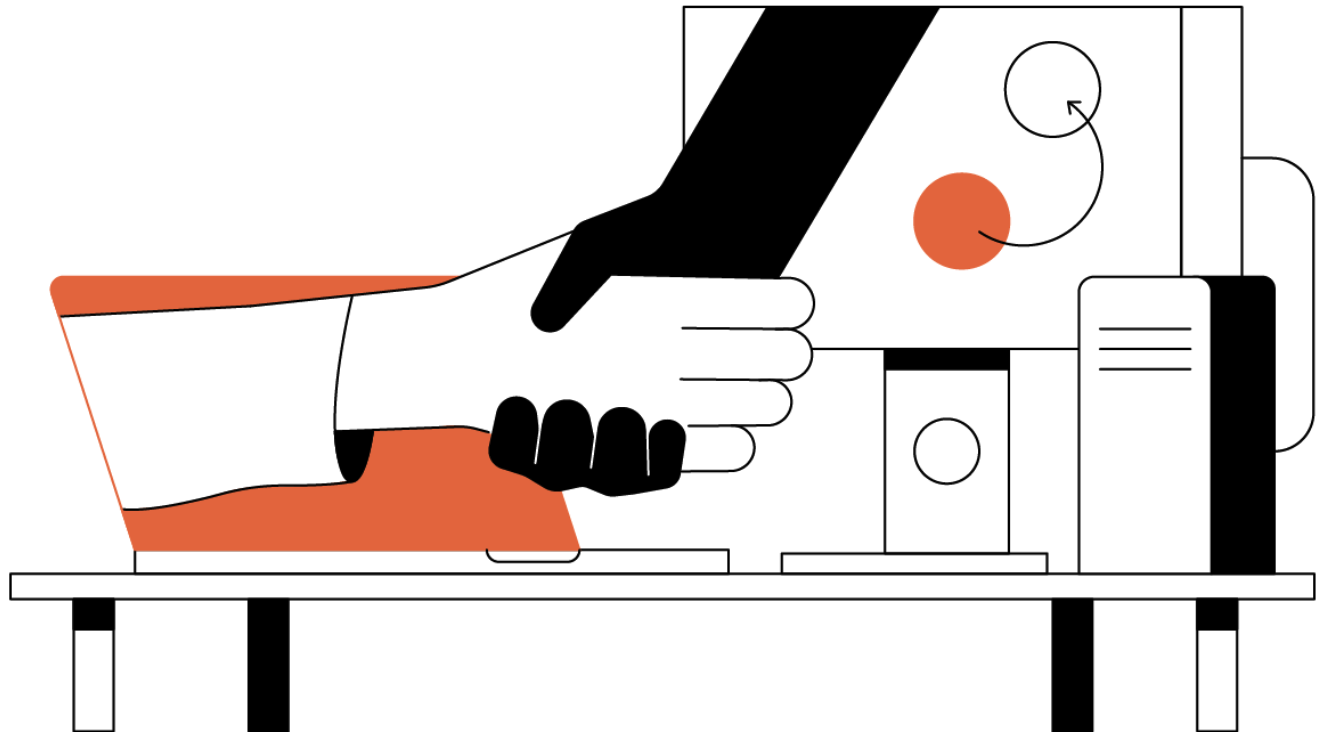
\includegraphics
		[width=0.6\textwidth]{assets/Gemini-What_Is_a_Decentralized_Exchange__DEX__.png}
		\caption{A
		decentralized
		exchange
		(DEX)
		\cite{-decentralized}}
		\label{fig: DEX}
	\end{teaserfigure}

	\received{20 February 2007} \received[revised]{12 March 2009} \received[accepted]{5 June 2009}

	%%
	%% This command processes the author and affiliation and title
	%% information and builds the first part of the formatted document.
	\maketitle


	\section{Introduction}


	Climate change and associated environmental concerns form the primary impetus for
	our project, with a focus on leveraging the transformative potential of
	decentralized exchanges (DEX) and blockchain solutions. Our overarching ambition
	is to contribute substantially to global climate change mitigation efforts.

	The urgency of addressing climate change cannot be overstated. As evidenced by
	\cite{-remaininga} , we are rapidly approaching the critical threshold of 1.5
	degrees of average warming, with less than 7.5 years remaining. Historical
	$CO_{2}$ concentration levels have risen dramatically from 280 parts per
	million (ppm) in the pre-industrial era to approximately 419 ppm at present
	due to fossil fuel combustion. With current projections estimating a rise by 2ppm
	per annum, we are fast nearing the critical level of 430 ppm, the point at which
	we hit 1.5 degrees of warming. In order to return to safe levels, there is a daunting
	task of removing nearly one trillion tons of $CO_{2}$ from the atmosphere.
	Hence, there is a pressing need for innovative solutions to mitigate climate change.

	The European Union (EU) has manifested its commitment to climate change mitigation
	by aiming for a 55\% reduction in greenhouse gas emissions by 2030 (compared to
	1990 levels), with a view to achieving net-zero emissions by 2050. As part of these
	efforts, the EU has introduced the Carbon Border Adjustment Mechanism (CBAM), which
	mandates importers to account for the emissions produced during the manufacturing
	of imported goods. Importers are required to obtain CBAM certificates
	corresponding to the volume of emissions associated with their imports, thereby
	contributing to the EU's ambitious carbon reduction targets and fostering sustainable
	practices in international trade.

	Notably, the chief purchasers of EU ETS offsets are corporations with
	emissions reduction obligations. These entities may opt to purchase offsets as
	a cost-effective alternative to reducing emissions within their own operations.
	CBAM, scheduled for implementation on October 1st, 2023, with full enforcement
	by 2026, aims to ensure that importers account for the emissions associated
	with their imported goods. The mechanism as shown in Table \ref{tab:comparison_of_different_mechanisms}
	encompasses several sectors, including cement, iron and steel, aluminium, fertiliser,
	electricity, polymers, organic chemicals, hydrogen, and ammonia. CBAM, by
	incorporating both direct and indirect emissions, unlike its predecessor, the
	ETS, aims to enforce a mandatory carbon price, thereby advancing the EU's
	annual emissions reduction target of 2.20\% to 4.20\%.

	\begin{table}[h]
		\caption{Comparison of different mechanisms}
		\begin{tabularx}
			{\linewidth}{|X|X|X|} \hline \textbf{Criteria} & \textbf{Option 1} &
			\textbf{Option 2} \\ \hline Annual emissions reduction target & 2.20\% &
			4.20\% \\ \hline Mechanism & Cap-and-trade & Mandatory carbon price \\ \hline
			Covered sectors & All sectors & Cement, iron and steel, aluminum,
			fertilizer, electricity, polymers, organic chemicals, hydrogen, ammonia \\
			\hline Emissions & Direct emissions only & Include indirect emissions \\ \hline
			Centralized authority & 27 competent authorities & One centralized EU CBAM
			authority \\ \hline Incentives & No & Yes \\ \hline
		\end{tabularx}
		\label{tab:comparison_of_different_mechanisms}
	\end{table}

	Given the EU's ambitious emissions reduction targets and the global impetus for
	sustainability, it is evident that emissions pricing is an effective mechanism
	to incentivize the reduction of carbon footprints. In light of this, we
	propose the development of a smart contract that employs a specialized
	approach to predict carbon pricing, which can support policy-making, promote
	compliance, and potentially catalyze the transition to a low-carbon economy.
	This tool would empower governments and regulatory bodies to assess the
	efficacy of existing policies and formulate new ones, while businesses could leverage
	it for regulatory compliance and environmental reporting.

	\section{Project Overview}


	The objective of this project is to delve into the development of a Uniswap-powered
	decentralized exchange designed for carbon trading. The paramount focus for
	the duration of this course will be on the third aspect of the project: Verification.
	This aspect embodies the creation of a certification and registry system for
	the transaction of carbon credits.

	The project revolves around four interwoven concepts: monitoring, reporting, verification,
	and trading. The primary goal is to orchestrate a system to track carbon emissions
	across supply chains, thus affording users the capacity to obtain precise
	information about the carbon emissions resultant from their operations. This knowledge
	will empower them to take informed steps towards reducing their environmental footprint.

	Further to this, the project seeks to furnish tools that facilitate users in
	the calculation of emissions, the comparison against industry norms, and the
	reporting of these emissions in adherence with prescribed guidelines. Through this,
	we aim to facilitate compliance with regulatory reporting mandates, whilst empowering
	our users to adopt a data-driven approach to the reduction of their carbon emissions.

	The verification facet of the project, which forms the crux of this course, involves
	the design of an accredited registry for the transaction of carbon credits.
	This seeks to provide a transparent and secure platform for the trading of
	these credits, which can be used as a mechanism to offset emissions. The
	ultimate goal is to promote the transition towards a lower-carbon economy.

	Lastly, the project endeavours to provide a suite of services such as product ratings,
	bid matching, and transaction facilitation, specifically geared towards the
	trading of sustainably sourced and carbon-neutral products. The overarching intention
	behind these services is to further the cause of sustainable practices,
	helping users attain their individual sustainability targets.

	In conclusion, this project has been conceived to address the urgent need for a
	comprehensive and efficient system for the monitoring, reporting, verification,
	and trading of carbon emissions and credits. Given the constraints of time,
	however, this course will concentrate on the critical aspect of verification within
	the broader project scope.

	\section{Blockchain Architecture Design}


	In the pursuit of developing a Uniswap-powered Decentralized Exchange for Carbon
	Trading, the architecture design for the project will leverage several cutting-edge
	technologies, which include a distributed ledger, smart contracts, and Internet
	of Things (IoT) devices for the acquisition of external grid emission factor data.
	However, within the time frame of this course, the focus will be primarily on
	the construction of a decentralized platform for carbon emissions trading.

	It is important to note that while ensuring the integrity and veracity of data
	through IoT devices is an imperative facet of the project, it does not form the
	primary focus of the present stage. Rather, the immediate attention is centred
	on the provision of a secure, transparent, and reliable platform for carbon trading.
	The aim is to foster the adoption of sustainable practices, thus making a valuable
	contribution to the ongoing global efforts to mitigate the adverse impacts of climate
	change.

	At this juncture, it is pertinent to highlight what this project will
	facilitate trading in, and how it introduces innovation to the realm of carbon
	emissions trading. A detailed exploration of these aspects will follow in
	subsequent sections of this report. The underlying objective remains the development
	of a system that is both robust and efficient, and which offers a new paradigm
	in the trading of carbon credits, promoting both environmental sustainability and
	regulatory compliance.

	\section{Present Trading Products and Tokenization}


	The current market for carbon emissions trading and tokenization is a vibrant,
	rapidly-evolving sector. A primary example of this is found in China, where a
	mandatory quota trading system is in place for key emission-producing
	enterprises. In tandem with quota trading, voluntary project-based offset
	trading also exists, providing flexibility for entities seeking to manage their
	carbon footprints.

	Tokenization presents a path to greater efficiency and accountability in the realm
	of carbon trading. Within this model, tokens become the representation of carbon
	credits and offsets, available for purchase, sale, or trade within the
	marketplace. This approach leads to a diversified portfolio of carbon products,
	and importantly, encourages sustainable business practices.

	While the field of carbon emissions trading and tokenization remains in its nascent
	stages, growth has been exponential. As an increasing number of countries and corporations
	pledge to shrink their carbon footprints, the demand for carbon credits and
	offsets is predicted to rise. Thus, the development of sustainable solutions, such
	as our proposed decentralized carbon emissions trading platform, is imperative
	to address the urgent problem of climate change.

	Among the plethora of products on offer, this project is especially interested
	in Carbon Index Tokens. These tokens provide an opportunity for a diversified
	portfolio of carbon products, mitigating risks linked to exposure to individual
	carbon products. Traded on carbon emissions markets, these tokens enhance both
	market accessibility and transparency.

	The allure of Carbon Index Tokens lies in their transparency, where the
	performance of the underlying carbon products can be monitored and verified, offering
	investors a lucid understanding of their investments. This transparency
	additionally aids investors in hedging against potential price fluctuations
	within the carbon market, thereby lowering exposure to market risks.

	Accessibility forms another major advantage of Carbon Index Tokens. They
	provide a route for investors, irrespective of their knowledge or resources,
	to engage in the carbon market. This simplifies the investment process in sustainable
	practices and aids the transition towards a low-carbon economy.

	In summary, Carbon Index Tokens furnish investors with a valuable instrument
	for long-term exposure to the potential growth of the carbon market. They further
	sustainable practices and contribute to mitigating climate change by fostering
	the progression towards a low-carbon economy.

	\section{Smart Contracts Structure }


	In the pursuit of creating a robust decentralized carbon trading platform, a
	carefully designed contract structure forms the backbone of our system, prioritising
	liquidity, efficient trading, and a seamless user experience.

	At the heart of our platform lies the COREarth ERC20 contract, a fundamental
	mechanism that underpins all transactional and trading activities on the
	platform. This smart contract furnishes the necessary functionalities to facilitate
	the tokenization and subsequent trading of carbon credits.

	To ascertain the provision of liquidity and efficient trading, the COREarth
	Router contract is implemented as an integral part of our platform. This contract
	streamlines the swapping of tokens, hence delivering an intuitive and seamless
	user experience.

	Complementing these central contracts, the COREarth Pair and COREarth Factory contracts
	are further embedded within our system. The Pair contract is instrumental in
	the pairing of tokens, while the Factory contract establishes a comprehensive framework
	for the genesis of new tokens.

	In essence, our platform's smart contract structure epitomizes a carefully
	calibrated system designed to offer liquidity, efficient trading, and a user-friendly
	experience in the burgeoning field of decentralized carbon trading.

	\subsection{COREarthPair Contract}


	In the context of the Uniswap V2 decentralized exchange protocol built on the
	Ethereum blockchain, the COREarthPair smart contract plays a central role.
	This section will elucidate the initialization process of the contract, delve into
	its primary functions, and shed light on a few auxiliary functions, all aimed at
	fostering a comprehensive understanding of the contract's functionality.

	\subsection{Contract Initialization}


	The initialization of the UniswapV2Pair contract comprises two main steps.
	Initially, within the constructor, the factory address is defined. This address
	corresponds to the UniswapV2Factory contract, tasked with the creation of new
	token pairs. Subsequently, the `initialize` function assigns the token0 and
	token1 addresses. These represent the pair of ERC20 tokens which are subject to
	trading.

	\subsection{Core Functions}


	The UniswapV2Pair contract is governed by three core functions, namely `mint`,
	`burn`, and `swap`. The `mint` function facilitates users in depositing tokens
	and receiving liquidity tokens in return. It computes the amount of liquidity
	to mint based on the reserves and provided token amounts, updates the reserves,
	and emits a Mint event. Contrarily, the `burn` function enables users to
	eliminate liquidity by burning their respective liquidity tokens. It calculates
	the amount of token0 and token1 to return, contingent on the user's pool share,
	updates the reserves, and emits a Burn event. Lastly, the `swap` function
	enables trades between token0 and token1. It establishes the input and output amounts
	based on the available reserves and desired output amount, updates the
	reserves, and emits a Swap event.

	\subsection{Auxiliary Functions}


	A suite of auxiliary functions is also incorporated within the UniswapV2Pair contract.
	For instance, the `getReserves` function returns the current reserves for token0
	and token1. Moreover, the `skim` and `sync` functions address disparities between
	the actual token balances and the recorded reserves. The `skim` function
	aligns balances with reserves, while the `sync` function aligns reserves with balances.

	In summary, the UniswapV2Pair smart contract is an essential element of the
	Uniswap V2 protocol. It regulates the primary functionalities of token pairs,
	such as minting and burning of liquidity tokens, as well as swapping tokens.
	Comprehending its inner workings is crucial to appreciate the decentralized
	exchange mechanism and the innovative strides brought forth by the Uniswap
	protocol.

	Two distinctive innovations are embedded within our system. Firstly, our
	tokenization targets the carbon index, which embodies a diversified portfolio of
	carbon products. Secondly, the Factory contract, while referencing the
	UniswapV2Pair contract, does not inherit from it but dynamically deploys Pair contracts
	for different token pairs as and when required.
	\section{COREarthFactory}


	The UniswapV2Factory contract serves as an indispensable element within the
	Uniswap V2 decentralized exchange ecosystem, enabling the creation and management
	of unique token pairs. This contract underpins the operation and liquidity
	management within the Uniswap V2 platform. In our application, it introduces a
	unique feature where the "feeToSetter" address can be assigned to a
	governmental body, paving the way for institutional oversight.

	\subsection{UniswapV2Factory Overview}


	The UniswapV2Factory contract initiates with a constructor that designates the
	initial feeToSetter address. This particular address possesses the privilege
	to amend fee-oriented configurations.

	A user can query the aggregate count of pairs created through the
	allPairsLength() function, providing a snapshot of the exchange's expansion over
	time. The pivotal function of the contract, createPair(), checks for the
	existence of a pair when presented with two distinct tokens. If non-existent,
	it generates a new UniswapV2Pair utilizing the create2 assembly method and
	initializes the pair with the sorted tokens. Upon creation, the contract
	updates the getPair mapping in both directions, introduces the pair into the allPairs
	array, and triggers a PairCreated event.

	The contract facilitates modification of the feeTo address, where platform fees
	are directed, via the setFeeTo() function, executable only by the feeToSetter.
	The feeToSetter address itself can be altered through the setFeeToSetter()
	function, a privilege reserved for the current feeToSetter.

	\subsection{COREarthFactory Contract and Fee Mechanism}


	Building upon the UniswapV2Factory at address 0x5, the COREarthFactory
	contract incorporates a protocol fee of 0.05\% which is toggleable. The fee is
	regulated by the "feeToSetter" address, which in our case, can be assigned to
	a governmental institution, thus incorporating an element of institutional oversight.

	On creating a new token pair using the "createPair" function, a fee of 0.30\% is
	levied on all trades. From this fee, 83.3\% (0.25\%) is apportioned to liquidity
	providers and the remaining 16.6\% (0.05\%) is directed to the "feeTo" address
	(if set).

	The "setFeeTo" function designates the "feeTo" address, the recipient of
	collected trade fees, while the "setFeeToSetter" function assigns the "feeToSetter"
	address, the regulator of the protocol fee and the entity authorized to alter
	the "feeTo" address.

	The "allPairsLength" function returns the length of the "allPairs" array which
	encapsulates information pertaining to all token pairs created on the platform.
	The "getPair" function computes the new liquidity tokens to be minted for the "feeTo"
	address.

	In essence, the COREarthFactory contract embeds a fee mechanism that
	encourages liquidity and incentivizes liquidity providers while ensuring
	appropriate fee collection and distribution. This mechanism fortifies the long-term
	sustainability and success of our decentralized carbon emissions trading platform.

	\section{COREarthRouter}


	The Uniswap V2 decentralized exchange plays host to an essential smart contract
	known as UniswapV2Router01, providing a simplified interface to Uniswap V2's
	core functionalities. These encompass adding and removing liquidity, swapping
	tokens, and calculating input and output amounts for trading pairs.
	Furthermore, UniswapV2Router02, an upgrade over its predecessor, introduces additional
	features and optimizations.

	\subsection{UniswapV2Router01 Overview}


	The UniswapV2Router01 contract is structured into seven primary sections:

	\begin{enumerate}
		\item Add Liquidity

		\item Remove Liquidity

		\item Swap Tokens

		\item Swap ETH

		\item Swap Exact Tokens for ETH

		\item Quote

		\item Get Amounts
	\end{enumerate}

	Each section is dedicated to a specific functionality. Sections 1 and 2 pertain
	to adding and removing liquidity via the 'addLiquidity', 'addLiquidityETH', 'removeLiquidity',
	and 'removeLiquidityETH' functions. Section 3 handles token-to-token swaps,
	while Section 4 is responsible for Ether-to-token and token-to-Ether swaps. Section
	5 addresses swapping tokens for an exact Ether amount, and Section 6 computes
	the output amount of a trade with the 'quote' function. Lastly, Section 7
	provides the 'getAmountsOut' and 'getAmountsIn' functions to calculate input
	and output amounts for trades.

	\subsection{UniswapV2Router02: An Upgraded Interface}


	The UniswapV2Router02 contract extends UniswapV2Router01's functionalities, offering
	a range of additional features:

	\begin{enumerate}
		\item Functions **`swapExactTokensForTokensSupportingFeeOnTransferTokens`** and
			**`swapExactETHForTokensSupportingFeeOnTransferTokens`** facilitate seamless
			trading of tokens with a built-in transfer fee mechanism, such as
			deflationary tokens.

		\item The function **`swapExactTokensForETH`** includes an optional **`address`**
			parameter to designate an Ether recipient, unlike its counterpart in
			UniswapV2Router01.

		\item The **`swapExactTokensForTokensWithRoute`** function allows users to set
			a custom route for their token swaps.

		\item The **`getAmountsOutExactETH`** function calculates the precise output
			tokens amount against a specific Ether input.

		\item The **`getAmountsOutExactTokens`** function computes the exact Ether output
			against a specific token input.
	\end{enumerate}

	To conclude, UniswapV2Router01 and UniswapV2Router02 contracts serve as indispensable
	elements within the Uniswap V2 decentralized exchange ecosystem. The upgraded
	UniswapV2Router02 contract enhances the user experience by offering additional
	features, making it a more comprehensive and flexible solution for interacting
	with the Uniswap V2 ecosystem.

	\section{Carbon Finance}


	The application of decentralized exchanges (DEX) to carbon trading provides a potential
	pathway to incentivize environmental sustainability and promote a greener economy.
	The platform designed in this study facilitates the smooth exchange of carbon
	credit tokens (Token A) and stablecoins (Token B). This section outlines the process
	and steps involved in implementing this system.

	The proposed procedure can be broken down into several steps:

	\begin{enumerate}
		\item \textbf{Factory Contract Deployment:} The initiation phase involves the
			establishment of the primary contract responsible for creating trading pairs.

		\item \textbf{Fee Manager Assignment:} A fee manager is designated to administer
			transaction fees, fostering a fair exchange environment.

		\item \textbf{Trading Pair Creation:} A new trading pair, comprising Token A
			and Token B, is established to facilitate the exchange of carbon credits and
			stablecoins.

		\item \textbf{Token Addresses Provision:} The contract addresses for both tokens
			are input into the system.

		\item \textbf{Pair Contract Deployment:} Subsequently, the Factory Contract
			deploys a new Pair Contract specific to the established trading pair.

		\item \textbf{Liquidity Addition:} Users deposit both Token A and Token B into
			the Pair Contract, providing the necessary liquidity for trading
			operations.

		\item \textbf{Liquidity Token Generation:} The Pair Contract, in turn, issues
			ERC20-compatible liquidity tokens to the users, representing their stake
			in the liquidity pool.

		\item \textbf{Trading Operation:} With the system adequately set up, users
			can now engage in token swaps, as well as adding or removing liquidity.

		\item \textbf{Token Swap:} Users have the option to exchange Token A for Token
			B, incurring a transaction fee of 0.3%.


		\item \textbf{Liquidity Management:} Users are enabled to deposit or withdraw
			additional tokens to or from the Pair Contract.

		\item \textbf{Underlying Tokens Return:} Upon opting to remove liquidity,
			users destroy their respective liquidity tokens, prompting the Pair Contract
			to return both Token A and Token B.
	\end{enumerate}

	This innovative approach to integrating carbon credit trading within a
	decentralized exchange allows users to engage with carbon finance effortlessly.
	By making carbon trading more accessible and streamlined, the platform
	promotes environmental sustainability and a shift towards a greener future. It
	also provides a foundation upon which policy makers and supervisory agencies can
	evaluate the effectiveness of current policies and develop new initiatives encouraging
	a low-carbon economy.

	\bibliographystyle{ACM-Reference-Format}
	\bibliography{DSAA5022_Final_Report}


	%%
	%% If your work has an appendix, this is the place to put it.
	\appendix
\end{document}
\endinput
%%
%% End of file `sample-authordraft.tex'.